\chapter{Measurements}\label{ch:measurements}

\section{Recordings}\label{sec:recordings}

The measurements were conducted in an anechoic chamber at DTU's Department of Electrical Engineering using a microphone placed one meter away from the struck object. To record the sounds we used Bruel \& Kjær's half inch pressure field microphone type 4192 and microphone preamplifier power supply type 5935L, as well as the 744T digital audio recorder from Sound Devices at 44100 Hz sampling frequency. The setup can be seen in figure \ref{fig:experiment}.

\begin{figure}[H]
  \centering
    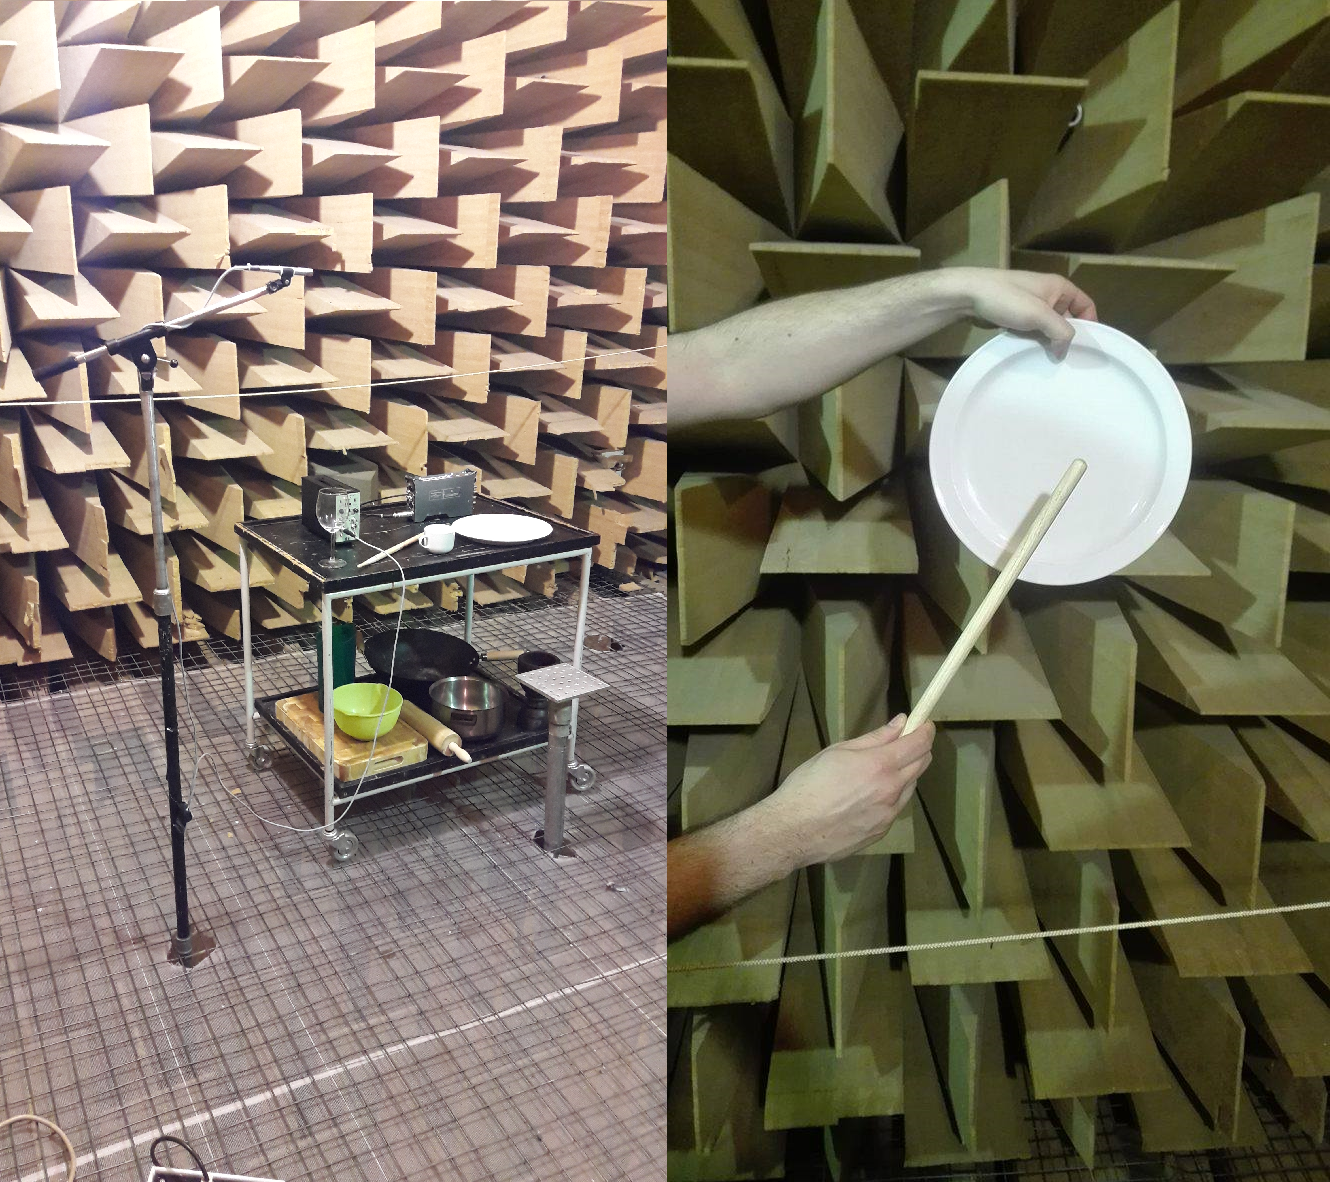
\includegraphics[width=0.6\textwidth]{experimentpic.png}
      \caption{Picture of the setup for the measurements (left) and of a struck object (right).}\label{fig:experiment}
\end{figure}

To control the impact we hit the objects by hand with a wooden drumstick (figure \ref{fig:experiment}) while trying to use the same impulsive force. Prior to the recordings, every object was divided into different surface areas depending on its shape and the sound produced by these areas. Therefore, several impact locations were chosen and recorded for every objects.

Eleven objects of everyday life made of five different materials (plastic, wood, ceramic, glass and metal) were used for the experiment. The idea of choosing these objects came firstly from the need of owning them (to perform the recording) and our ability to model them for the demo (as they should be simple enough). Secondly, since we wished to test the immersion of the synthesized sounds on users, we wanted to be sure that the sounds used are familiar to them. In figure \ref{fig:objects} both real and modeled objects are shown. 

\begin{figure}[H]
    \centering
    \begin{subfigure}[b]{0.7\textwidth}
        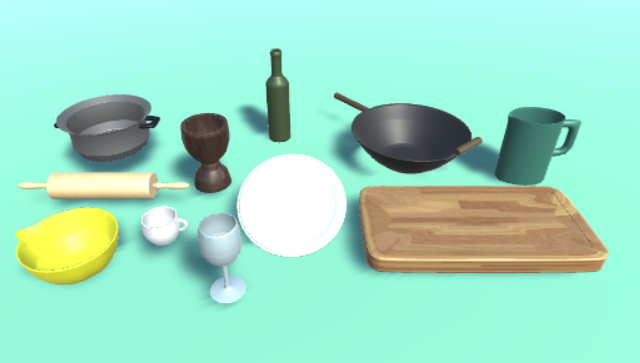
\includegraphics[width=\textwidth]{realobjects.PNG}
        \caption{Real objects.}
        \label{fig:gull}
    \end{subfigure}
    ~ %add desired spacing between images, e. g. ~, \quad, \qquad, \hfill etc. 
      %(or a blank line to force the subfigure onto a new line)
    \begin{subfigure}[b]{0.7\textwidth}
        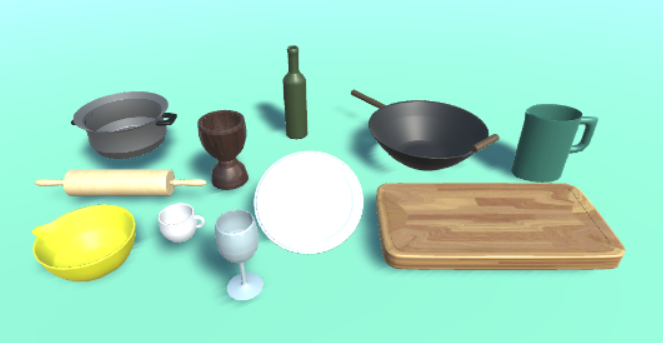
\includegraphics[width=\textwidth]{3dobjects.PNG}
        \caption{3D models of the objects.}
        \label{fig:tiger}
    \end{subfigure}
    \caption{The eleven objects used in the thesis.}\label{fig:objects}
\end{figure}

\section{User tests}\label{sec:tests}
When working on a field where human perception plays a significant role, it is important to test whether your work makes sense for target users and if it solves successfully the problem that was designed for.

To examine the immersion of real-time produced and physics-based sounds on game players, we performed \textit{MUSHRA}\cite{series2014method} tests to people. Our aim was to answer the following questions: \begin{inparaenum}[1)]
\item Which of the two synthesis methods (sinusoidal and filter-based additive synthesis) is closer to reality? 
\item Which is the range (in Q-factor values) of every material's sound?
\item Does physics-based synthesis make a sound more realistic and less boring?
\end{inparaenum}.

\subsection{Preparation}
For the tests we used several .wav files that we recorder inside the Unity\textregistered platform. We designed two special scenes for this purpose, because we wanted to test the sounds both in real-life conditions -when an object is falling and colliding with other objects- and the impulse response of the synthesis model (figure \ref{fig:test_scenes}). 

\begin{figure}[H]
    \centering
    \begin{subfigure}[b]{0.45\textwidth}
        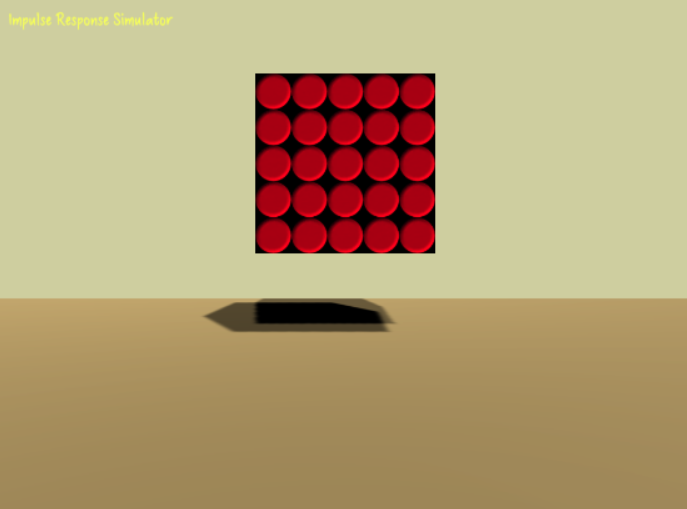
\includegraphics[width=\textwidth]{impulsescene.PNG}
        \caption{Impulse Response Simulator Scene.}
        \label{fig:test_sc1}
    \end{subfigure}
    ~ %add desired spacing between images, e. g. ~, \quad, \qquad, \hfill etc. 
      %(or a blank line to force the subfigure onto a new line)
    \begin{subfigure}[b]{0.45\textwidth}
        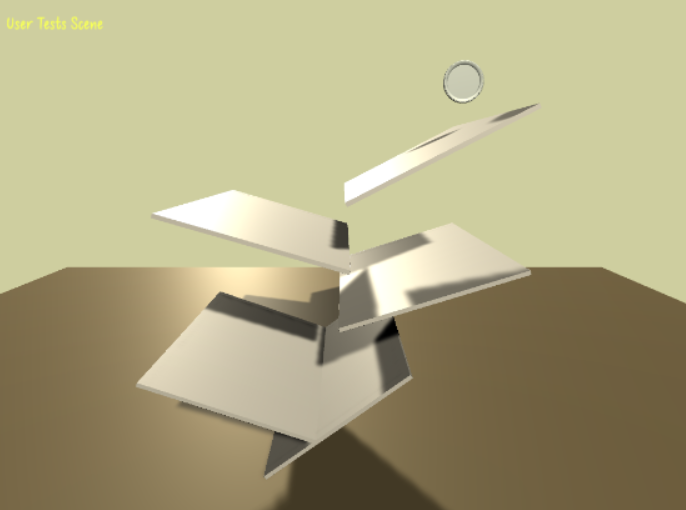
\includegraphics[width=\textwidth]{usertestscene.PNG}
        \caption{Real-Life Conditions Scene.}
        \label{fig:test_sc2}
    \end{subfigure}
    \caption{The Unity Scenes designed to record the .wav files used for the user tests.}\label{fig:test_scenes}
\end{figure}

In the first scene (figure \ref{fig:test_sc1}), we recorded the audio files for the first experiment. During the recording session, we ``tagged'' the cube as different objects (a process that assigns to the cube different modal data) and let it touch the ground without any bounce. We also repeated the process with an Audio Source and the recordings files, to achieve consistency of the stimuli.

In the second scene (figure \ref{fig:test_sc2}), we recorded the audio files for the second and third experiment. In this scene, objects fall, roll and scratch freely on rotated platforms, simulating a real room with obstacles.

\subsection{Stimuli}
We performed three different tests. On the first test, the stimuli was 44 pairs of impulse responses (one for each synthesis method) corresponding to different areas of the eleven materials and their corresponding reference sounds which were the recordings of the actual sounds produced by the physical objects. 

On the second test, the stimuli consisted of 33 pairs of sounds that were produced by falling objects. From the pair, one sound is produced when objects are split into ``sound areas'' and each area produces a different sound and the other sound is produced when every point of the objects makes the same sound. This single sound was the one produced from the area of each object where the recording taken (section \ref{sec:recordings}) was closer to the real sound of this object in our opinion.  

The stimuli of the third test was 50 sounds coming from five different objects, one of each material under testing (plastic jug, wooden mortar, ceramic plate, glass bottle and metallic cooking pot). For each object, we used 10 different sounds that corresponded to a small variation on the Q-factor which changes the material of the object. More specifically, starting from a value of 600, we increased the Q-factor by 200 up to 4600, removed some sounds that were too similar with others and provided participants with the rest.

\subsection{Procedure}
Stimuli was presented to the participants through \Todo{describe headphones}, in a room with reduced external noise.

In the first test, participants were provided with a reference sound (the actual recording) and two testing sounds (the sinusoidal and filter-based synthesized sounds), and they were asked to choose the one sounding closer to the reference. In the second test, participants were given pairs of sounds where the first one was made of multiple sounds per area of the object and the second one was made by the same sound assigned to every area. They were asked to answer which of the two they prefered. Finally, in the third test, they were provided with sounds from the same object but with different materials assigned to it and they were asked to point out when a change in material happens. 

Every sound file starts 1 second after participant presses play and ends half a second after no sound can be heard.

\subsection{Participants}
\Todo{number of participants, age, gender, normal hearing, job}

\subsection{Test Results}